%%% Variables, functions and other settings
%% Define document class and theme
\documentclass{beamer}
\usetheme{Goettingen}
%% Define basic variables
\title{Bootcamp}
\subtitle{Getting sprint 0 started!}
\author{Team 11}
\institute[]{
  Project 2 \\
  Toolbox for managing the training \\
  neural networks (Pyry Takala) \\[0.3cm]
  CSE-C2610 Software Project \\
  Aalto University
}
\date{14th Oct 2015}
\subject{Software engineering}
%% Logo
% Replace navigation symbols with a logo
\logo{
\includegraphics[height=1cm]{../gfx/logo_aalto.png}}
\setbeamertemplate{navigation symbols}{\insertlogo}
%% Functions
% Define short set and clear background commands
\newcommand{\bgset}[1]{\usebackgroundtemplate{
  \includegraphics[width=\paperwidth,height=\paperheight]{#1}}}
\newcommand{\bgclear}{\usebackgroundtemplate{}}
% Have LaTeX render an outline frame just before each new section/subsection
\AtBeginSection[]{
  \bgset{../gfx/neural4__bgmod.jpg}
  \begin{frame}<beamer>{Outline}
    \tableofcontents[currentsection]
  \end{frame}
  \bgset{../gfx/neural3__bgmod.jpg}}
\AtBeginSubsection[]{
  \bgset{../gfx/neural4__bgmod.jpg}
  \begin{frame}<beamer>{Outline}
    \tableofcontents[currentsection,currentsubsection]
  \end{frame}
  \bgset{../gfx/neural3__bgmod.jpg}}
%%% Main document content
\begin{document}
%% Title page
\bgset{../gfx/neural2__bgmod.jpg}
\begin{frame}
  \titlepage
\end{frame}
%% Outline page
\bgset{../gfx/neural4__bgmod.jpg}
\begin{frame}{Outline}
  \tableofcontents[pausesections]
\end{frame}
%% Content pages
\section{Things to do}
\subsection{Overview}
\begin{frame}{Overview}
  Things to do in Sprint 0:
  \begin{enumerate}
  \pause \item Make drafts of required artifacts.
  \pause \item Review them with the team
  \pause \item Review them with the coach
  \pause \item Review them with the PO
  \pause \item Interview other researchers and IT staff
  \pause \item Finish the artifacts
  \pause \item Get ready for sprint 1
  \end{enumerate}
\end{frame}
\subsection{Artifacts}
\begin{frame}{Artifacts}
  Artifacts to prepare:
  \begin{enumerate}
  \pause \item Product Vision
  \pause \item Product \& Sprint Backlog
  \pause \item Process Overview
  \pause \item Technical Overview
  \pause \item Definition of Done
  \pause \item Progress/Final Report
  \pause \item Learning Diary
  \pause \item Test Session Charter
  \end{enumerate}
  \pause \alert{Enough work} \pause for \alert{everyone}, huh!?
\end{frame}
\bgset{../gfx/neural1__bgmod.jpg}
\begin{frame}{Product Vision}
  \begin{itemize}
  \item relatively easy
  \item why, what and for whom
  \item improved with the PO
  \end{itemize}
  Workload: 3 hours of pairwork for a good draft.
\end{frame}
\begin{frame}{Product \& Sprint Backlog}
  \begin{itemize}
  \item more cumbersome
  \item need to learn about Trello \\
    Our team: \url{https://trello.com/sdpt11} \\
    Should also check these:
    \href{http://scrumfortrello.com/}{a},
    \href{http://www.tommasonervegna.com/blog/2014/1/9/10-effective-tips-for-using-trello-as-an-agile-scrum-project-management-tool}{b}
  \item Workflow:
    \begin{enumerate}
    \item create product \& sprint backlogs in Trello
    \item add user stories and items like "design an architecture"
    \item meet PO for review
    \end{enumerate}
  \end{itemize}
  Workload: 3 hours of pairwork?
\end{frame}
\begin{frame}{Process Overview}
  \begin{itemize}
  \item involves lots of decisions
  \item needs input from all team mates
  \item probably takes a lot of time
  \end{itemize}
  Workload: 6 hours of pairwork?
\end{frame}
\begin{frame}{Technical Overview}
  \begin{itemize}
  \item involves brainstorming, googling and making charts
  \item misdesigns get fixed as we learn more
  \end{itemize}
  Workload: 3 hours of pairwork?
\end{frame}
\begin{frame}{Definition of Done}
  \begin{itemize}
  \item involves some decisions
  \item otherwise easy
  \end{itemize}
  Workload: 3 hours of pairwork?
\end{frame}
\begin{frame}{Other artifacts}
  The remaining artifacts aren't needed yet:
  \begin{itemize}
  \item Progress/Final Report
  \item Learning Diary
  \item Test Session Charter
  \end{itemize}
  Should be kept in mind though.
\end{frame}
\section{How to do them}
\subsection{Notes}
\begin{frame}{Notes}
  Some notes:
  \begin{enumerate}
  \pause \item Scheduling meetings is difficult! \\
  \pause It takes time and not everyone is able to attend.
  \pause \item Independent working is effective! \\
  \pause 10\% team + 50\% mate + 40\% alone, remember?
  \pause \item We agreed to aim for grade 5! \\
  \pause I'd rather use \alert{less} than more time! \\
  ~ How about you?
  \end{enumerate}
  \pause So let's get working shall we!
\end{frame}
\subsection{Ideas}
\begin{frame}{Ideas}
  Ideas:
  \begin{itemize}
  \pause \item Let's define subteams! \\
  \pause Swap coordination for more useful discussion \& work done!
  \pause \item Let's share work to subteams! \\
  \pause Clear distribution of workload + clear DL = results effectively!
  \pause \item Let's have subteam peer-review! \\
  \pause More discussion \& better results while still effective!
  \end{itemize}
  \pause \alert{Hmmh..?}
\end{frame}
\begin{frame}{Process}
  \begin{figure}
    \centering
    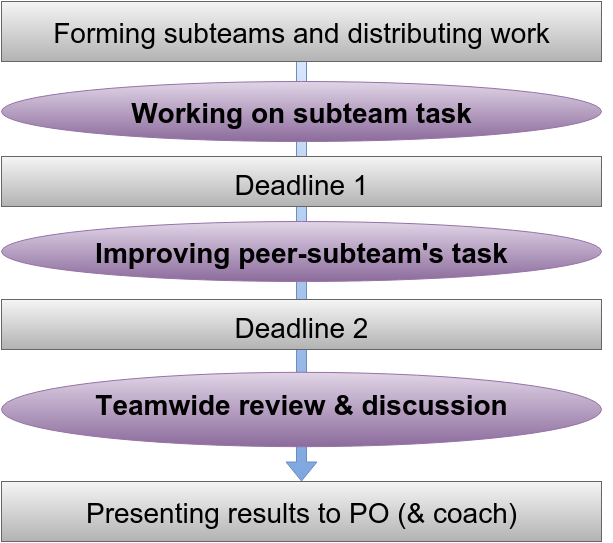
\includegraphics[width=0.8\columnwidth]{../gfx/subteam_process.png}
  \end{figure}
\end{frame}
\subsection{Subteams}
\begin{frame}{Subteams}
  How about:
  \begin{table}
  \begin{tabular}{lll}
  ID & Members & Peer-reviewer \\ \hline
  \texttt{joju} & Joona \& Juho & \texttt{iima} \\
  \texttt{tetu} & Teemu \& Tuomo & \texttt{joju} \\
  \texttt{iima} & Iiro \& Matias & \texttt{tetu} \\
  \end{tabular}
  \end{table}
  \pause Note that we could change the subteams periodically so that everyone
  gets to really know everyone else well. Plus:
  \begin{itemize}
  \pause \item You get to learn how others work and choose the best methods.
  \pause \item With a mate, many things are a lot easier!
  \end{itemize}
  \pause It's about balancing team\alert{power} and team\alert{waste}: \\
  $1 + 1 \approx 2.5$ but $8 ~\textrm{min} \times 7 \approx 1 ~\textrm{hour}$
\end{frame}
\subsection{Work allocation}
\begin{frame}{Work allocation}
  How about we distribute the work thus:
  \begin{table}
  \begin{tabular}{lll}
  Work & Workload & Team \\ \hline
  \pause Product Vision & 3 & \texttt{joju} \\
  \pause Pro./Sprint Backlog & 3 & \texttt{tetu} \\
  \pause Process Overview & 6 & \texttt{iima} \\
  \pause Technical Overview & 3 & \texttt{tetu} \\
  \pause Definition of Done & 3 & \texttt{joju} \\
  \end{tabular}
  \end{table}
  \pause Fair?
\end{frame}
\subsection{Timeline} \bgset{../gfx/neural1__bgmod.jpg}
\begin{frame}{Timeline}
  \begin{figure}
    \centering
    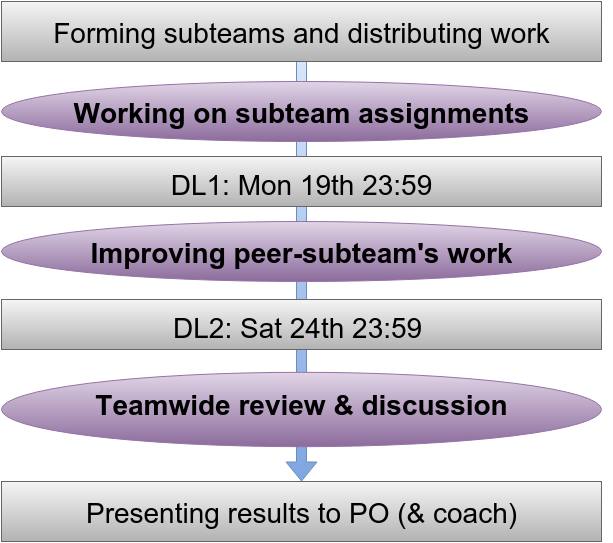
\includegraphics[width=0.8\columnwidth]{../gfx/subteam_process_fixed.png}
  \end{figure}
\end{frame}
\section*{Summary}
\begin{frame}{Summary}
  Main points:
  \begin{itemize}
  \pause \item We've got a lot to do
  \pause \item Meetings with PO \& coach are more useful when we are prepared
  \pause \item Pairwork with peer review is the way to go
  \pause \item It's better to start working now
  \end{itemize}
\end{frame}
\section*{Discussion}
\begin{frame}{Discussion}
  Thanks for your patience! \\[1cm]
  What did/do you think?
\end{frame}
\end{document}
